\chapter{\todo{Decapolar Fields}}
\label{chapter:decapoles}
\thumbforchapter{}
%\chaptertoc{}
%\newpage

% === Introduction
\section{\review{Introduction}}

% -----------------------
%       Motivation
\subsection{\review{Motivation}}

Beam-based measurements have been carried in the LHC since Run 1 to better understand the decapolar
fields. Those have been carried out via chromaticity
measurements~\cite{maclean_non-linear_2011,maclean_commissioning_2016,maclean_measurement_2014}. 
The third order of the non-linear chromaticity, $Q'''$, generated for the most part by decapoles,
has shown a consistent discrepancy at injection energy between its expected value from simulations
and that observed. Figure \ref{fig:decapoles:bare_chroma_vs_simulations} highlights this
discrepancy.

\begin{figure}[!htb]
    \centering
    \includegraphics[width=0.8\textwidth]{images/dq3_corrected_simulation_fidel.pdf}
    \caption{Measured and simulated chromaticity with application of the nominal decapolar
    corrections from FiDeL. It can be seen that although the corrections should diminish $Q'''$, it
    is not well corrected in practice.}
    \label{fig:decapoles:bare_chroma_vs_simulations}
\end{figure}

The FiDeL magnetic model is used during operation to correct various multipole errors, including
octupolar and decapolar. The operational corrections being based on this magnetic model and
simulations, the residual $Q'''$ value is expected to be small, which is however not the case.
Chromaticity measurements have thus been repeated during LHC's Run 3 and corrections made routine,
aimed at correcting the observed discrepancy.

The study of non-linear chromaticity has proven valuable in quantifying decapolar fields, yet it
does not permit alone to understand the exact origins of the observed discrepancy. In an effort to
gain deeper insights, additional measurements were performed focusing on novel observables that had
not been previously explored.
\textit{Bare chromaticity} involves measuring chromaticity with
the octupolar an decapolar correctors deactivated ; this approach aims to isolate the machine
effects from those of the correctors.
\textit{Chromatic amplitude detuning}, evaluates how the tune varies with both the beam's action and
the momentum offset ; this methods has the benefit of having a different expression that of the
chromaticity.

Complementing those measurements, studies of decapolar Resonance Driving Terms have been undertaken
for the first time in the LHC. Contributing to resonances close to the working, those RDTs also have
benefited from corrections.


% --------------------------
%    Decapolar Correctors
\subsection{\review{Decapolar Correctors}}

As seen in \cref{fig:introduction:lhc_arc_cell}, the LHC is equipped with decapoles. Those magnets
are part of the design report, aiming at correcting the field errors of the main dipoles.
Those correctors, denominated \textit{MCD}, are specific to each beam and are placed after every
second dipole, totaling 1232 in number~\cite{venturini_delsolaro_magnetic_2005}.
MCDs are nested with octupolar correctors, \textit{MCO}. The pair of those correctors of often
referred to as \textit{MCDO}. 
It is not possible to individually power each corrector. Rather, a circuit consists of a whole arc.
There are in total 16 circuits to control the correctors of both beams and 8 arcs.
\cref{fig:decapoles:decapole_picture} shows a picture taken of decapoles on a test bench.

\begin{figure}
    \centering
    \includegraphics[width=0.4\textwidth]{./images/decapoles_real_pic.jpg}
    \caption{Decapoles on a test bench, being inspected after
    manufacturing~\cite{noauthor_ten_2001}.}
    \label{fig:decapoles:decapole_picture}
\end{figure}


The important characteristics of the magnetic fields of correctors are their main field transfer
function (or \textit{response}), the field quality and possible crosstalk, as MCOs and MCDs are
nested~\cite{venturini_delsolaro_magnetic_2005}.
In order to better understand the decapolar fields, the decapole correctors themselves need to be
studied.


% -------- Strengths at Injection
\paragraph{Strengths at Injection}

%\begin{wraptable}{r}{0.4\textwidth}
\begin{table}
    \centering
    \begin{tabular}{lr}
        \toprule
        Circuit   & $K_5 [\textrm{m}^{-5}]$ \\
        \midrule
        Beam 1    & \\
        \hspace{2mm}RCD.A12B1 & $-4582$ \\
        \hspace{2mm}RCD.A23B1 & $-5106$ \\
        \hspace{2mm}RCD.A34B1 & $-4855$ \\
        \hspace{2mm}RCD.A45B1 & $-4577$ \\
        \hspace{2mm}RCD.A56B1 & $-4125$ \\
        \hspace{2mm}RCD.A67B1 & $-5166$ \\
        \hspace{2mm}RCD.A78B1 & $-6827$ \\
        \hspace{2mm}RCD.A81B1 & $-5500$ \\
        Beam 2    & \\
        \hspace{2mm}RCD.A12B2 & $-4490$ \\
        \hspace{2mm}RCD.A23B2 & $-5155$ \\
        \hspace{2mm}RCD.A34B2 & $-4825$ \\
        \hspace{2mm}RCD.A45B2 & $-4619$ \\
        \hspace{2mm}RCD.A56B2 & $-4064$ \\
        \hspace{2mm}RCD.A67B2 & $-5066$ \\
        \hspace{2mm}RCD.A78B2 & $-6866$ \\
        \hspace{2mm}RCD.A81B2 & $-5446$ \\
        \bottomrule
    \end{tabular}
    \caption{Strength of decapolar correctors at injection energy for FiDeL corrections.}
    \label{tab:decapoles:strength_rcd_fidel}
%\end{wraptable}
\end{table}

At injection energy, the decapoles are powered to a static strength. New optics introduced
throughout the years often have for effect to vary slightly the $\beta$-function along the ring,
having thus an impact on the chromaticity, as seen in
\cref{eq:detuning_effects:chromaticity_strength}. New corrections are then computed via FiDeL to
account for it.
Although those corrections vary throughout the years, the shift is in practice fairly negligible.
\cref{tab:decapoles:rdts:correction_f1004_k5}, a bit further in this chapter, shows the strength of
the correctors and the related circuits at injection energy for the optics deployed in 2024.


%==================================
%          Chromaticity
%==================================
\section{Non-Linear Chromaticity}

Measurements were taken during 2022 Commissioning for 
\begin{itemize}
    \item Beam Test
    \item Commissioning
    \begin{itemize}
        \item FiDeL
        \item Q''' corr
        \item Q'' corr
    \end{itemize}
    \item 60° optics
\end{itemize}

Also during MD6864, 2022-10-19, for the bare machine \\
Also 2022-11-06, measurement at 30cm, flat top.



%==================================
%   Chromatic Amplitude Detuning
%==================================
% ###################################
%      Chromatic Amplitude Detuning
\section{\review{Chromatic Amplitude Detuning}}

The Chromatic Amplitude Detuning is the tune shift dependant on both the actions and the momentum
offset, whose decapole contributed terms are described via a Taylor expansion in
\cref{eq:decapoles:chromatic_ampdet:decapole_contribution}. More information and derivations can
be found in \cref{subsection:detuning_effects:chromatic_amplitude_detuning} and
\cref{appendix:chromatic_amplitude_detuning}.

\begin{equation}
  \begin{aligned}
    \Delta Q(J_x, J_y, \delta) = 
    & \frac{\partial^2Q}{\partial J_x \partial \delta}    \cdot J_x\delta 
    + \frac{\partial^2 Q}{\partial J_y \partial \delta}   \cdot J_y\delta 
    + \frac{1}{3!} \frac{\partial^3 Q}{\partial \delta^3} \cdot \delta^3.
    \end{aligned}
    \label{eq:decapoles:chromatic_ampdet:decapole_contribution}
\end{equation}


The last term is more commonly referred to as the third order chromaticity, $Q'''$.  Each of those
terms depend on the $\beta$-functions, the horizontal dispersion $D$ and the normalized decapole
field gradient $K_5$ for a single source of length $L$,

\begin{equation}\begin{aligned}
  \frac{\partial^2 Q_x}{\partial J_x \partial \delta} =& \frac{1}{16 \pi} K_5L \beta_x^2 D,         &\quad
  \frac{\partial^2 Q_x}{\partial J_y \partial \delta} =& -\frac{1}{8\pi} K_5L \beta_x \beta_y D,
\\
  \frac{\partial^3 Q_x}{\partial \delta^3}            =& \frac{1}{4\pi} K_5L \beta_x D^3,           &\quad
  \frac{\partial^2 Q_y}{\partial J_x \partial \delta} =& -\frac{1}{8\pi} K_5L \beta_x \beta_y D,
\\
  \frac{\partial^2 Q_y}{\partial J_y \partial \delta} =& \frac{1}{16 \pi} K_5L \beta_y^2 D,        &\quad 
  \frac{\partial^3 Q_y}{\partial \delta^3}            =& -\frac{1}{4\pi} K_5L \beta_y D^3.
\end{aligned}\end{equation}

The action dependant terms can be measured by exciting the beam with an AC-dipole with increasing
strengths at different momentum-offsets.

Such a measurement was taken with octupole and decapole correctors turned off to measure the bare
machine. Some data could not be collected due to machine availability issues, restricting the
measurement to low intensity kicks. 
Nevertheless, the terms $\frac{\partial^2 Q_x}{\partial J_y \partial \delta}$ and $\frac{\partial^2
Q_y}{\partial J_y \partial \delta}$ for beam 2 were measured for the first time in the LHC. The
momentum-offsets measured at were $-0.001$ and $0.001$, respectively roughly equal to a trim of 
$+140$Hz and $-140$Hz of the RF.

\cref{figure:decapoles:chromatic_amplitude_detuning:b2qxy}
and~\cref{figure:decapoles:chromatic_amplitude_detuning:b2qyy} show a fit of those terms to measured
$Q_{x,y}$ vs $J_{y}$ at two different momentum offsets. Expected shifts from MADX-PTC simulations,
that include field errors ranging from sextupoles to decahexapoles ($b_3$ to $b_8$ and $a_4$ to
$a_8$) are shown as a comparison.

% Studies and plots in 
% jupyter/chromatic_amplitude_detuning/simulations/2022-10-19_vs_PTC/Analytical_Chromatic_Detuning.ipynb

\begin{figure}[H]
  \centering
  \begin{subfigure}{0.8\textwidth}
      \centering
      \includegraphics[width=\textwidth]{images/chromatic_amplitude_detuning/B2_Qxy_decay0.00.pdf}
      \caption{Horizontal tune shift depending on the vertical action: 
      $\frac{\partial^2 Q_x}{\partial J_y \partial \delta}$.}
      \label{figure:decapoles:chromatic_amplitude_detuning:b2qxy}
  \end{subfigure}
  %
  \\[1em]
  %
  \begin{subfigure}{0.8\textwidth}
      \centering
      \includegraphics[width=\textwidth]{images/chromatic_amplitude_detuning/B2_Qyy_decay0.00.pdf}
      \caption{Vertical tune shift depending on the vertical action: 
      $\frac{\partial^2 Q_y}{\partial J_y \partial \delta}$.}
      \label{figure:decapoles:chromatic_amplitude_detuning:b2qyy}
  \end{subfigure}
  \caption{Measured and simulated tune shift due to a change of action via an AC-Dipole at two
  different momentum offsets. Each fit corresponds to a chromatic amplitude detuning term evaluated
  at a certain $\delta$.}
  \label{figure:decapoles:chromatic_amplitude_detuning:two_terms}
\end{figure}


\begin{table}[H]
  \centering
  \begin{tabular}{lrr}
  \toprule
   Type  & $\frac{\partial^2 Q_x}{\partial J_y \partial \delta}[10^{4}\mathrm{m}^{-1}]$ & $\frac{\partial^2 Q_y}{\partial J_y \partial \delta}[10^{4}\mathrm{m}^{-1}]$ \\
  \midrule
  $\delta = +0.001$ & & \\
  \hspace{2mm}Meas.  &   -1.16 ± 0.08 &   1.26 ± 0.15 \\
  \hspace{2mm}Sim.   &   -3.82 ± 0.01 &   2.47 ± 0.01 \\
  \hspace{2mm}Ratio  &    0.30 ± 0.02 &   0.51 ± 0.06 \\
  $\delta = -0.001$ & & \\
  \hspace{2mm}Meas.  &  1.47 ± 0.12  &  -1.18 ± 0.13 \\
  \hspace{2mm}Sim.   &  3.92 ± 0.01  &  -2.41 ± 0.01 \\
  \hspace{2mm}Ratio  &  0.38 ± 0.03  &   0.49 ± 0.05 \\
  \bottomrule
  \end{tabular}
  \caption{Comparison of the measured and simulated terms $\frac{\partial^2 Q_x}{\partial J_y
   \delta}$ and $\frac{\partial^2 Q_y}{\partial J_y \partial \delta}$ via PTC, at two
  discrete momentum offsets. Simulations include errors from normal sextupole to decahexapole and
  from skew octupole to decahexapole.}
  \label{table:decapoles:chromatic_ampdet}
\end{table}



A consistent difference between simulation and measurement is observed, which values and
ratios of measurement to model can be found in \cref{table:decapoles:chromatic_ampdet}.
The observed ratios of measurement to model for the chromatic amplitude detuning show slight
discrepancies compared to the bare chromaticity ones. These discrepancies could be due to the low
intensity kicks, which don't allow for a better fit. However, the similarity of the ratios suggests
an issue with the decapolar error model of the main dipoles, with measurements showing values about
half of those predicted by the magnetic model.


%==================================
%              Decay 
%==================================
%==================================
%              Decay 
%==================================
\section{\review{Accounting for Decay}}
\label{section:decapoles:decay}

FiDeL, the field model used in operation, aims at correcting the field errors at various energies.
Measured field errors but also decay estimates with respect to time are used when computing
corrections.

Magnetic decay in superconducting magnets stems from field changes in the strands caused by current
redistribution in the superconducting cables. Decay has been shown to be strongly dependent on the
magnet powering history~\cite{sammut_dependence_2006,haverkamp_studies_1999}.
This happens for example when ramping down from an energy of 6.8TeV to 0 and then going back to
injection energy at 450GeV. Some components of the magnetic field will persist and gradually change
over time until they reach their final value.

While the sextupolar $b_3$ decay is accounted for during operations, a review of the FiDeL model
revealed that the decapolar component $b_5$ has not been similarly considered. To date, all beam
dynamics studies in the LHC have made use of the same set of magnetic measurement error tables, thus
neglecting any decapolar decay. It has though be found that during the LHC construction, magnetic
measurements were taken for a representative set of main dipoles, and decay measured.
%
The average $b_5$ field in the main dipoles at $t=0$, upon reaching the 450 GeV energy, is
approximately $1.145 \pm 0.5$, based on data from the magnetic reports utilized by FiDeL. For
reference, decay measurements of a selection of main dipoles over time are illustrated in
\cref{fig:decapoles:decay:decay_b5}.
%
\Cref{table:decapoles:decay:decay_b5} shows the decay expected at injection energy after a typical
cycle of machine operation. From this table, it is clear that decay accounts for a large part of the
$b_5$ at injection. $\approx 40\%$ of the compensated $b_5$ at injection in the main dipoles can
indeed be attributed to the decay.

\begin{figure}[!htb]
    \centering
    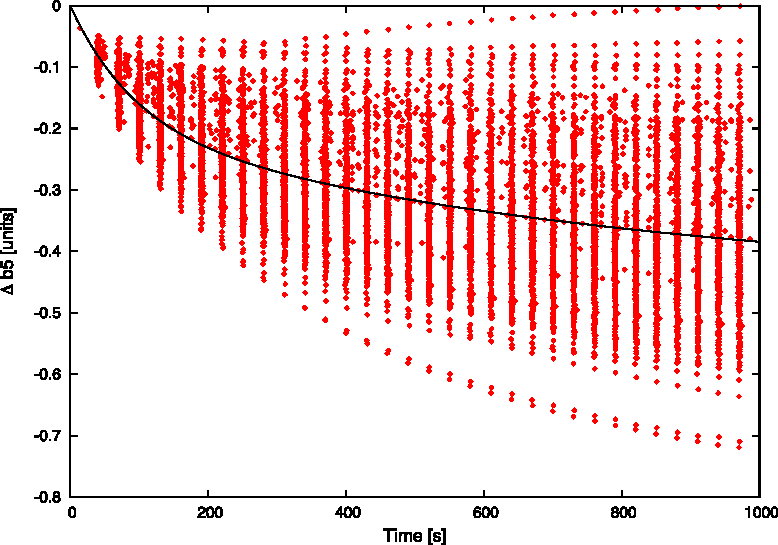
\includegraphics[width=0.7\textwidth]{./images/decay_b5_mb.pdf}
    \caption{Measured decay of the integrated decapolar field in LHC's main dipoles at injection
    energy. The fit is shown in black~\cite{deniau_magnetic_2009}.}
    \label{fig:decapoles:decay:decay_b5}
\end{figure}

\begin{table}[!htb]
    \centering
    \begin{tabular}{cl}
        \toprule
        Time [m] & $\Delta b_5$ \\
        \midrule
        $17$    & -0.38 \\ 
        $33$    & -0.44 \\
        $50$    & -0.46 \\
        $67$    & -0.47 \\
        $83$    & -0.47 \\
        $167$   & -0.47 \\
        \bottomrule
    \end{tabular}
    \caption{Decay of the $b_5$ component after injection for long time
    periods~\cite{deniau_magnetic_2009}.}
    \label{table:decapoles:decay:decay_b5}
\end{table}
 
Unfortunately, individual magnet measurements conducted over 15 years ago could not be recovered. As
a result, the $b_5$ decay in the simulations is implemented as the average decay across all the
probed magnets. In the following simulations, each main dipole sees its $b_5$ component reduced by
$0.47$ units.


% ==== Chromaticity
\paragraph{Chromaticity}

It has been shown in the previous sections, and particularly in
\cref{table:decapoles:bare_chromaticity:virgin_dq3} that measurements and simulations were off
regarding the third order chromaticity $Q'''$.
New simulations have hence been conducted to evaluate the effect of this decay on chromaticity.
\Cref{table:decapoles:decay:simulation_chromaticity} compares simulations with and
without the decay of the $b_5$ component. The simulations use the 100 available error seeds to
calculate error bars.

\begin{table}[!htb]
    \centering
    \begin{tabular}{lll}
      \toprule
      Condition            & $Q'''_x [10^6]$ & $Q'''_y [10^6]$ \\
      \midrule
      No Decay             & $6.93 \pm 0.04$ & $-4.32 \pm 0.02$ \\
      $\Delta b_5 = -0.47$ & $4.05 \pm 0.04$ & $-2.54 \pm 0.02 $ \\
      \bottomrule
    \end{tabular}
    \caption{Comparison of $Q'''_x$ and $Q'''_y$ for Beam 1 with and without decay of the $b_5$
    component of the main dipoles at injection energy. Fields errors range from normal and skew
    sextupoles ($n=3$) to icosapole ($n=10$).}
    \label{table:decapoles:decay:simulation_chromaticity}
  \end{table}

Implementing the decay of the $b_5$ component of the main dipoles in the simulations have
significantly reduced the discrepancy between beam-based measurement and the magnetic model.
%
Using the values from the bare chromaticity measurement and updating
\cref{table:decapoles:bare_chromaticity:virgin_dq3} with the newly obtain data provides a more
accurate description of the magnetic model, as shown in
\cref{table:decapoles:decay:virgin_dq3_recompare}.


\begin{table}[!htb]
    \centering
    \begin{tabular}{rrrr}
      \toprule
      Quantity     &  Measured $[10^6]$        &  Simulated $[10^{6}]$          &   \multicolumn{1}{c}{Ratio}     \\
      \midrule
        \multicolumn{1}{l}{Beam 1}    &                             &                                &             \\
                $Q'''_x$ &       $ 2.95 \pm 0.04$      & $ 4.05 \pm 0.04$               &  $0.73 \pm 0.01$  \\
                $Q'''_y$ &       $-1.82 \pm 0.04$      & $-2.54 \pm 0.02$               &  $0.72 \pm 0.02$  \\
      %\midrule
        \multicolumn{1}{l}{Beam 2}    &                             &                                &             \\
                $Q'''_x$ &       $ 3.06 \pm 0.07$      & $ 4.27 \pm 0.03$               &  $0.72 \pm 0.02$  \\
                $Q'''_y$ &       $-1.72 \pm 0.02$      & $-2.55 \pm 0.01$               &  $0.67 \pm 0.01$ \\
      \bottomrule
    \end{tabular}
    \caption{Measured and simulated third order chromaticity with octupole and decapole correctors
    turned off. The simulations include field errors from normal and skew sextupoles to icosapole
    ($n=3$ to $n=10$). The $b_5$ component of the main dipoles has been updated to include decay.}
    \label{table:decapoles:decay:virgin_dq3_recompare}
\end{table}




% ==== Chromatic Amplitude Detuning
\paragraph{Chromatic Amplitude Detuning}

Similar to chromaticity, new simulations have been conducted for chromatic amplitude detuning.
\Cref{table:decapoles:decay:chromatic_ampdet} gives an overview of the newly computed values and 
the related ratios relative to the measurements, while \cref{figure:decapoles:decay:two_terms} gives
a visual clue.
A small difference in agreement can be observed between the direct term $\partial^2 Q_y / (\partial
J_y \partial \delta)$ and the crossterm. This may arise from the implementation of decay, which only
considers the average $b_5$ across all dipoles and may not fully capture the individual variations.
Nevertheless, both terms now demonstrate good agreement with the model, similar to the trend seen
with chromaticity.


\begin{table}[H]
  \centering
  \begin{tabular}{lrr}
  \toprule
   Type  & $\frac{\partial^2 Q_x}{\partial J_y \partial \delta}[10^{4}\mathrm{m}^{-1}]$ & $\frac{\partial^2 Q_y}{\partial J_y \partial \delta}[10^{4}\mathrm{m}^{-1}]$ \\
  \midrule
  $\delta = +0.001$ & & \\
  \hspace{2mm}Meas.  &   $-1.16 \pm 0.08$ &  $1.26 \pm 0.15$  \\
  \hspace{2mm}Sim.   &   $-2.35 \pm 0.01$ &  $1.50 \pm 0.01$  \\
  \hspace{2mm}Ratio  &   $ 0.49 \pm 0.03$ &  $0.84 \pm 0.10$  \\
  $\delta = -0.001$ & & \\
  \hspace{2mm}Meas.  &  $1.47 \pm 0.12$  &   $-1.18 \pm 0.13$ \\
  \hspace{2mm}Sim.   &  $2.46 \pm 0.01$  &   $-1.45 \pm 0.01$ \\
  \hspace{2mm}Ratio  &  $0.60 \pm 0.05$  &   $ 0.82 \pm 0.09$ \\
  \bottomrule
  \end{tabular}
  \caption{Comparison of the measured and simulated terms $\frac{\partial^2 Q_x}{\partial J_y
  \partial \delta}$ and $\frac{\partial^2 Q_y}{\partial J_y \partial \delta}$ via PTC, at two
  discrete momentum offsets. Simulations include errors from normal and skew sextupoles to 
  icosapole ($n=3$ to $n=10$), as well as the decay of the $b_5$ component of the main dipoles.}
  \label{table:decapoles:decay:chromatic_ampdet}
\end{table}

\begin{figure}[H]
  \centering
  \begin{subfigure}{0.8\textwidth}
      \centering
      \includegraphics[width=\textwidth]{images/chromatic_amplitude_detuning/B2_Qxy_decay0.47.pdf}
      \caption{Horizontal tune shift depending on the vertical action: 
      $\frac{\partial^2 Q_x}{\partial J_y \partial \delta}$.}
      \label{figure:decapoles:decay:b2qxy}
  \end{subfigure}
  %
  \\[1em]
  %
  \begin{subfigure}{0.8\textwidth}
      \centering
      \includegraphics[width=\textwidth]{images/chromatic_amplitude_detuning/B2_Qyy_decay0.47.pdf}
      \caption{Vertical tune shift depending on the vertical action: 
      $\frac{\partial^2 Q_y}{\partial J_y \partial \delta}$.}
      \label{figure:decapoles:decay:b2qyy}
  \end{subfigure}
  \caption{Measured and simulated tune shift depending on the action at two different momentum
  offsets. Each fit corresponds to a chromatic amplitude detuning term evaluated at a certain
  $\delta$. Estimates from simulations are lowered due to the $b_5$ decay of the main dipoles.}
  \label{figure:decapoles:decay:two_terms}
\end{figure}




%==================================
%      Resonance Driving Terms
%==================================
% === RDTs
\section{Resonance Driving Terms}

Decapoles, due to their order, contribute to many RDTs. Indeed, 50 of them can be theoretically 
observed in simulations and measurements. In practice, the contributions of individual RDTs
become indistinguishable as many resonances overlap, making it impossible to isolate certain terms.
Up to a fixed order, some resonances, described in~\cref{appendix:rdts}, are unique to
certain multipoles. Those resonances, provided that they are sufficiently strong and close to the
beam, can be measured via their RDTs.

Of interest to the LHC Operation, is the RDT $f_{1004}$, driving the resonance $1Q_x - 4Q_y$.
It can be seen in the horizontal frequency spectrum at $-4Q_y$ with an amplitude dependence on
$J_y^2$. 
Figure~\cref{fig:decapoles:rdts:tune_diagram} shows a frequency
map~\cite{yannis_papaphilippou_detecting_nodate} of a simulation including decapolar field errors,
where their impact on the beam is easily noticeable. The \todo{red} particles evolving close to the
resonance are affected by it and are subject to large tune shifts. Eventually, those particles are 
lost when their amplitude becomes too large.

\begin{figure}[H]
    \centering
    \includegraphics[width=0.8\textwidth]{./images/tune_diagram_f1004.pdf}
    \caption{Frequency map at injection energy, with decapolar field errors and nominal settings for
    landau octupoles. The highlighted resonance (1,-4), excited by decapoles, shows a degradation
    over 20,000 turns. The tune shift between the start and the end of the simulation is indicated
    in colour. \todo{change colormap}}
    \label{fig:decapoles:rdts:tune_diagram}
\end{figure}

Measuring turn-by-turn data without using any excitation is not a viable option as amplitudes are
not large enough. Spectral lines are indeed usually impossible to discern from the noise floor, 
making RDTs not measurable.
Measurements are hence taken with an AC-Dipole, introducing quadrupolar-like field errors in the 
linear regime~\cite{carlier_nonlinear_2020} and more complex effects in the non linear regime.
In practice, those effects are neglected. \textit{Forced} RDTs are measured with an
AC-Dipole and treated as \textit{free} as no compensation is applied.

Such forced measurements were taken for the first time in the LHC to observe the $f_{1004}$ RDT
at injection energy. The frequency line of the resonance $1Q_x - 4Q_y$ is seen at $4Q_y$ in the
horizontal spectrum, as shows \cref{fig:decapoles:rdts:spectrum_f1004}.

\begin{figure}[H]
    \centering
    \includegraphics[width=0.9\textwidth]{./images/f1004x_spectrum.pdf}
    \caption{Horizontal frequency spectrum of turn-by-turn data, with nominal and beam-based
    corrections for the third order chromaticity $Q'''$. The $1Q_x - 4Q_y$ resonance can be seen
    at $-4Q_y$ with different amplitudes for each correction scheme.}
    \label{fig:decapoles:rdts:spectrum_f1004}
\end{figure}

Moreover, \cref{fig:decapoles:rdts:spectrum_f1004} shows that the amplitude of this resonance line
decreases upon application of beam-based corrections for $Q'''$. This translates to the amplitude
of the RDT $f_{1004}$, as seen in \cref{fig:decapoles:rdts:f1004_dq3}.

\begin{figure}[H]
    \centering
    \includegraphics[width=0.9\textwidth]{./images/f1004_dq3.pdf}
    \caption{Amplitude of the RDT $f_{1004}$ generated by normal decapoles, measured before and
    after having applied beam-based corrections of the third order chromaticity $Q'''$.}
    \label{fig:decapoles:rdts:f1004_dq3}
\end{figure}


\todo{
    Measurements: \\
    \begin{itemize}
        \item 2022 Q'' and Q''' corrections 2022-04-24
        \item 2022-10-19 Virgin machine
        \item 2023-easter (FiDeL)
        \item 2023-06-14 MD9549 (FiDeL and Q'''/ RDT corr)
    \end{itemize}
    Effect of RCO correction on RDT f1004 \\
    Response
}

% ---------------------------------------
%         Decapole Contribution
% ---------------------------------------
\subsection{\todo{Decapolar Contribution}}


% ---------------------------------------
%        Higher Order Contribution
% ---------------------------------------
\subsection{\review{Higher Order Contributions}}

% Measurements in 
% /afs/cern.ch/work/m/mlegarr2/public/beta_beat_output/2024-05-21

To produce collisions at top energy, \textit{crossing angles} are introduced via the orbit
correctors located in the triplets, before the separation dipoles and the matching section of the
interaction regions (\texttt{MCBX}, \texttt{MCBY} and \texttt{MCBC})~\cite{de_maria_lhc_2008}. Those
collisions happen with a small $\beta*$, currently 30cm, requiring strong quadrupolar fields from
the triplets.

At such $\beta$, those triplets also generate strong dodecapolar field errors. Because of the
crossing-angles, feed-down appears and lower-order fields can be observed.
Such feed-down to decapolar fields was observed during the first commissioning of Run~3, in
2022~\cite{maclean_prospects_2022}.
\cref{fig:decapoles:f1004_from_feeddown} shows how the RDT $f_{1004}$, normally affected by
decapoles, varies with the application of crossing angles.

\begin{figure}[H]
    \centering
    \includegraphics[width=0.9\textwidth]{./images/f1004x_feed-down_b6_triplets.pdf}
    \caption{}
    \label{fig:decapoles:f1004_from_feeddown}
\end{figure}

Such a contribution is though not expected at injection energy, as the triplets aren't powered as
much as at top energy, $\beta*$ being set at around $10$m.

% ---------------------------------------
%        Lower Order Contribution
% ---------------------------------------
\subsection{\todo{Lower Order Contributions}}

% http://localhost:8888/lab/workspaces/auto-d/tree/work_afs2/jupyter/resonance_driving_terms/measurements/2024-03-13_b3_b4_effect_on_b5/Sextupoles_and_Octupoles.ipynb

% ------- Introduction
\subsubsection{\review{First Observation}}

As described in \cref{appendix:transfer_maps}, multipoles can combine to create fields that are seen
as higher orders when considering higher orders of the BCH expansion.
For decapoles, combinations of several sextupoles and sextupoles with octupoles give rise to
decapolar-like fields, as described in
\cref{table:appendix:transfer_maps:bch_resulting_orders_combination}. The following parts of this
section will describe those combinations.

This effect was observed in 2022 during Run 3's commissioning. Routine corrections of the non-linear
chromaticity $Q''$ and $Q'''$ were performed, and RDT measurements taken before and after their
correction. As $Q'''$ was corrected, the expectation was that the RDT $f_{1004}$ would also lower
with the reduction of the decapolar strengths $K_5$. However, an increase of the RDT was observed,
as shows \cref{fig:decapoles:f1004_dq2_dq3}.

\begin{figure}[H]
    \centering
    \includegraphics[width=0.9\textwidth]{./images/f1004_dq2_dq3_2022.pdf}    
    \caption{Non intuitive increase of the RDT $f_{1004}$ after application of the $Q''$ and $Q'''$
    corrections.\todo{redo plot}}
    \label{fig:decapoles:f1004_dq2_dq3}
\end{figure}


% ------- Action dependance
\subsubsection{\review{Action Dependance and Analysis}}

Resonance lines in the frequency spectrum are often contributed to by several multipoles. Some lines
start getting a contribution with rather high multipole orders, like the RDT $f_{1004}$ considered
here. The line $4Q_y$ in the horizontal spectrum is indeed contributed to by decapoles and then only
by decatetrapoles. When the main contributing field alone is varied, it is easy to reconstruct the
RDT, as its fit is only dependant its action dependance ($\propto J_x^{*} J_y^{*}$). Several
turn-by-turn measurements at the same configuration can be taken wit varying kick amplitudes,
refining the RDT value with more data points for the fit.

Considering the contribution of lower order multipoles is a bit trickier, as the second order RDTs
change the dependance of the frequency line~\cite{franchi_first_2014}. In order to be able to
extract the RDT from several turn by turn measurements, the same kick amplitude must then be used.

%\todo{simulation plot of varying amplitudes for Q' = 2 and noise created from it}

% ------- Sextupoles
\subsubsection{\todo{Sextupoles}}

At the third order of the BCH expansion, the combination of two sextupoles yields a decapolar-like
expression. Derivation of such a combination can be found in
\cref{appendix:transfer_map:two_sextupoles}. The resulting Hamiltonian indeed is similar to
the terms of a decapole, dropping the $p_{x,y}$ terms for readability:

\begin{equation}
    \begin{aligned}
         (H_3)^3 &\propto \frac{1}{48} \left(x^5 - 2x^3y^2 - 3xy^4 \right)\\
                 &\sim    x^5 - 10x^3y^2 + 5xy^4.
    \end{aligned}
\end{equation}

This means that, during normal operation of the machine, decapolar observables will be altered when
adjusting parameters such as the linear chromaticity $Q'$. A simulation was run with injection
optics and varying the linear chromaticity $Q'$. The resulting effect on the RDT $f_{1004}$ can be
seen in \cref{decapoles:rdts:simulated_f1004_from_sextupoles}.

\begin{figure}[H]
    \centering
    \includegraphics[width=0.9\textwidth]{./images/f1004/f1004_dq.pdf}
    \caption{Simulated change of the decapolar RDT $f_{1004}$ depending of the desired linear
    chromaticity $Q'$ generated by sextupoles.}
    \label{decapoles:rdts:simulated_f1004_from_sextupoles}
\end{figure}



\cref{decapoles:rdts:measured_f1004_from_sextupoles} shows measurements done with varying values
for $Q'$. 

\begin{figure}[H]
    \centering
    \includegraphics[width=0.9\textwidth]{./images/f1004/f1004x_q2_q10_q15.pdf}
    \caption{Measured change of the decapolar RDT $f_{1004}$ depending of the desired linear
    chromaticity $Q'$ generated by sextupoles.}
    \label{decapoles:rdts:measured_f1004_from_sextupoles}
\end{figure}

%Measurements are typically performed at $Q' = 3$

% ------- Sextupole + Octupole
\subsubsection{\todo{Sextupoles and Octupoles}}

\begin{figure}[H]
    \centering
    \includegraphics[width=0.9\textwidth]{./images/f1004/f1004_mo.pdf}
    \caption{Simulated change of the decapolar RDT $f_{1004}$ depending of the landau octupoles 
    (\texttt{MO}) strength.}
    \label{}
\end{figure}

\begin{figure}[H]
    \centering
    \includegraphics[width=0.9\textwidth]{./images/f1004/f1004_no_ms.pdf}
    \caption{Simulated decapolar RDT $f_{1004}$ with two different schemes. First scheme has
    lattice sextupoles turned off and octupoles turned on. Second scheme has all sextupoles of the
    lattice turned off and octupoles turned off as well. No difference is seen, as expected from
    the equations.}
    \label{}
\end{figure}

\begin{figure}[H]
    \centering
    \includegraphics[width=0.9\textwidth]{./images/f1004/f1004x_mco_corr.pdf}
    \caption{Different MCO Corr.}
    \label{decapoles:rdts:measured_f1004_mco}
\end{figure}


%==================================
%             Impact
%==================================
% === Impact / Lifetime
\FloatBarrier
\section{\review{Impact of Decapolar Fields}}

Decapolar fields can influence the beam lifetime in several ways. Chromatic amplitude detuning and
chromaticity will induce a tune shift, relative to either or both the action and the momentum
offset. After such detuning, particles may move closer to certain resonances in tune space, causing
their oscillations to grow, eventually leading to their loss.


% ============================================
%                 Large RDT
% ============================================
\subsection{\review{Large RDT}}

\begin{wraptable}{r}{0.4\textwidth}
    \centering
    \begin{tabular}{rr}
    \toprule
    $\Delta K_5$         & RMS $|f_{1004}|$ \\
    \midrule
    $0$                  &            $618,947$ \\
    $\pm10500$             &         $17,566,377$ \\
    $\mp10500$             &         $17,623,867$ \\
    \bottomrule
    \end{tabular}
    \caption{RMS of $|f_{1004}|$ relative to the powering scheme of decapolar correctors.}
    \label{table:decapoles:impact:rdt_amplitude}
\end{wraptable}

As seen previously in \cref{fig:decapoles:rdts:tune_diagram}, the resonance $1Q_x - 4Q_y$ passes
through the beam in tune space, deteriorating the lifetime of the nearby particles.
In order to measure the impact of this resonance on the beam, a knob was created, alternating the 
current of all decapole correctors in the machine arc by arc. Such a powering scheme has no impact
on chromaticity as the sum of the strengths $K_5$ is zero. Rather, the RDT $f_{1004}$ is impacted.
Is it to be noted that this is not a correction, but purely a way to artificially increase the RDT
in order to quantify the effect of the resonance.

Starting with nominals corrections for $Q'''$ corrections, a delta of $\pm 10500 K_5$ is applied on
each decapolar correctors. \Cref{fig:decapoles:impact:alternating_knob} shows the response of the
real part of the RDT for this scheme and its inverse. The amplitude of the RDT is on a similar level
as the shift is significantly larger than the original level of the RDT.
\Cref{table:decapoles:impact:rdt_amplitude} indicates the amplitude of the RDT created with each
knob value.

\begin{figure}[!htb]
    \centering
    \includegraphics[width=0.8\textwidth]{./images/f1004/f1004x_knob_alt_lifetime_real.pdf}
    \caption{Measured real part of the RDT $f_{1004}$ depending on the powering scheme of the decapolar
    correctors.}
    \label{fig:decapoles:impact:alternating_knob}
\end{figure}

In order to measure the lifetime, a long period must be allocated as the signal returned from
monitors can be jittery. \Cref{fig:decapoles:impact:b5_lifetime} shows this lifetime depending on
the decapolar strength scheme applied. The current of only one circuit is shown for readability.
A current of $\approx 230$ corresponds to a knob value of $+10500$ while a current of $-45$
corresponds to $0$.

\begin{figure}[!htb]
    \centering
    \includegraphics[width=0.8\textwidth]{./images/b5_lifetime.pdf}
    \caption{Measured lifetime of Beam 2 upon application of two different powering schemes for
    decapolar correctors. One trim keeps the RDT at a low amplitude while the other greatly
    amplifies it.}
    \label{fig:decapoles:impact:b5_lifetime}
\end{figure}

It is clear from this measurement that a large RDT decreases the lifetime of the beam.
The first pair of trim sees the average lifetime decreasing of $0.31 \pm 0.03$ hours, while the
second one sees a decrease of $0.36 \pm 0.03$ hours. This observed decrease of 20 minutes accounts
for $10\%$ of the beam lifetime at injection energy.



% ============================================
%                Corrections
% ============================================
\subsection{\review{Corrections}}

In order to understand what can be gained from correcting decapolar fields, a lifetime measurement
was taken with the corrections described in 
\cref{section:decapoles:decapolar_contribution_correction}. This scheme corrects the three decapolar 
observables, being the RDT $f_{1004}$ linked to the resonance $1Q_x - 4Q_y$, the third order
chromaticity $Q'''$ and the chromatic amplitude detuning terms.
\Cref{fig:decapoles:impact:b5_lifetime_rdt_corr} shows the evolution of the lifetime, starting with
corrections applied, removed and then trimmed to their opposite. A net change in lifetime for Beam 1
can be measured after each application. Acquired signal for Beam 2 has been deemed too noisy to be 
relevant, due to the shortness of the measurement.

\begin{figure}[!htb]
    \centering
    \includegraphics[width=0.8\textwidth]{./images/b5_lifetime_rdt_corr.pdf}
    \caption{Measured lifetime of Beam 1 with the nominal corrections for $Q'''$, combined
    correction of $f_{1004}$ and $Q'''$, and its inverse.}
    \label{fig:decapoles:impact:b5_lifetime_rdt_corr}
\end{figure}

It is apparent here that the corrections have a beneficial effect on the beam. The lifetime
improvement is of $\approx 3 \%$, while the degradation after applying the opposite is of $\approx
5\%$. Further developments in the correction scheme and lengthier measurements could easily improve
this lifetime gain.


Furthermore, a significant improvement in the forced dynamic aperture during AC-Dipole excitation
was observed when corrections were applied. The earlier corrections for decapolar fields were
implemented alongside octupolar corrections for $Q''$. \Cref{fig:decapoles:losses_b4b5_corrs}
demonstrates the relative losses encountered when kicking at different amplitudes with the
AC-Dipole. This clearly shows that octupolar and decapolar corrections enhance the forced dynamic
aperture.

\begin{figure}[!htb]
    \centering
    \includegraphics[width=0.8\textwidth]{./images/losses_with_without_b4b5corr.pdf}
    \caption{Relative losses experienced with AC-Dipole kick amplitude with and without corrections
    pertaining to $Q''$, $Q'''$, chromatic amplitude detuning, and RDT $f_{1004}$.}
    \label{fig:decapoles:losses_b4b5_corrs}
\end{figure}

\FloatBarrier


%==================================
%            Summary
%==================================
\section{\todo{Summary}}

blabla